\documentclass[11pt,a4paper]{article}
\usepackage[margin=2.3cm]{geometry}
\usepackage{microtype}
\usepackage{amsmath,amssymb}
\usepackage{booktabs}
\usepackage{graphicx}
\usepackage{xcolor}
\usepackage{enumitem}
\usepackage[font=small,labelfont=bf]{caption}
\usepackage[colorlinks=true,linkcolor=blue!50!black,citecolor=blue!50!black,urlcolor=blue!50!black]{hyperref}
\newcommand{\numBelowRange}{91}
\newcommand{\numCandidatesTest}{240}
\newcommand{\numCandidatesValidation}{216}
\newcommand{\numCellFrozenOldCbSelAcc}{77.8}
\newcommand{\numCellFrozenOldCbSharedAcc}{77.6}
\newcommand{\numCellFrozenOldShSelAcc}{47.6}
\newcommand{\numCellFrozenOldShSharedAcc}{46.2}
\newcommand{\numCellFrozenOldShSharedForg}{55.7}
\newcommand{\numCellOrdinaryCbSelAcc}{77.3}
\newcommand{\numCellOrdinaryCbSharedAcc}{76.9}
\newcommand{\numCellOrdinaryShSelAcc}{62.6}
\newcommand{\numCellOrdinaryShSharedAcc}{56.8}
\newcommand{\numCellOrdinaryShSharedForg}{43.7}
\newcommand{\numErBestAcc}{75.7}
\newcommand{\numErBestAccSd}{1.1}
\newcommand{\numErBestForg}{17.0}
\newcommand{\numErBestForgSd}{2.2}
\newcommand{\numErBestNew}{77.4}
\newcommand{\numErBestParams}{13{,}834}
\newcommand{\numErBestTime}{0.71}
\newcommand{\numErCandidates}{35}
\newcommand{\numErFloorTradeAcc}{75.7}
\newcommand{\numErFloorTradeAccSd}{0.5}
\newcommand{\numErFloorTradeForg}{12.4}
\newcommand{\numErFloorTradeForgSd}{1.4}
\newcommand{\numErFloorTradeNew}{71.9}
\newcommand{\numErFloorTradeParams}{6{,}922}
\newcommand{\numErFloorTradeTime}{0.29}
\newcommand{\numErHindAcc}{76.0}
\newcommand{\numErHindAccSd}{0.9}
\newcommand{\numErHindForg}{13.2}
\newcommand{\numErHindForgSd}{1.9}
\newcommand{\numErHindNew}{72.7}
\newcommand{\numErHindParams}{13{,}834}
\newcommand{\numErHindTime}{0.59}
\newcommand{\numErLinearAcc}{66.8}
\newcommand{\numErLinearAccSd}{0.2}
\newcommand{\numErLinearForg}{13.1}
\newcommand{\numErLinearForgSd}{0.5}
\newcommand{\numErLinearNew}{59.5}
\newcommand{\numErLinearParams}{170}
\newcommand{\numErLinearTime}{0.12}
\newcommand{\numErLowForgAcc}{74.7}
\newcommand{\numErLowForgAccSd}{0.3}
\newcommand{\numErLowForgForg}{10.3}
\newcommand{\numErLowForgForgSd}{1.4}
\newcommand{\numErLowForgNew}{67.5}
\newcommand{\numErLowForgParams}{6{,}922}
\newcommand{\numErLowForgTime}{0.32}
\newcommand{\numErNoReplayAcc}{18.8}
\newcommand{\numErNoReplayAccSd}{0.1}
\newcommand{\numErNoReplayForg}{96.5}
\newcommand{\numErNoReplayForgSd}{0.2}
\newcommand{\numErNoReplayNew}{93.9}
\newcommand{\numErNoReplayParams}{13{,}834}
\newcommand{\numErNoReplayTime}{0.67}
\newcommand{\numErTenBestAcc}{76.0}
\newcommand{\numErTradeAcc}{72.3}
\newcommand{\numErTradeAccSd}{0.3}
\newcommand{\numErTradeForg}{10.4}
\newcommand{\numErTradeForgSd}{1.0}
\newcommand{\numErTradeNew}{64.0}
\newcommand{\numErTradeParams}{1{,}738}
\newcommand{\numErTradeTime}{0.19}
\newcommand{\numFeatureSeconds}{15.8}
\newcommand{\numFloorCandidates}{76}
\newcommand{\numHHERBesttradeoffAcc}{75.7}
\newcommand{\numHHERBesttradeoffAccSd}{0.5}
\newcommand{\numHHERBesttradeoffForg}{12.4}
\newcommand{\numHHERBesttradeoffForgSd}{1.4}
\newcommand{\numHHERBesttradeoffNew}{71.9}
\newcommand{\numHHERBesttradeoffParams}{6{,}922}
\newcommand{\numHHERBesttradeoffTime}{0.29}
\newcommand{\numHHERHighestaccuracyAcc}{76.0}
\newcommand{\numHHERHighestaccuracyAccSd}{0.9}
\newcommand{\numHHERHighestaccuracyForg}{13.2}
\newcommand{\numHHERHighestaccuracyForgSd}{1.9}
\newcommand{\numHHERHighestaccuracyNew}{72.7}
\newcommand{\numHHERHighestaccuracyParams}{13{,}834}
\newcommand{\numHHERHighestaccuracyTime}{0.59}
\newcommand{\numHHERLinearheadAcc}{66.8}
\newcommand{\numHHERLinearheadAccSd}{0.2}
\newcommand{\numHHERLinearheadForg}{13.1}
\newcommand{\numHHERLinearheadForgSd}{0.5}
\newcommand{\numHHERLinearheadNew}{59.5}
\newcommand{\numHHERLinearheadParams}{170}
\newcommand{\numHHERLinearheadTime}{0.12}
\newcommand{\numHHERLowestforgettingAcc}{74.7}
\newcommand{\numHHERLowestforgettingAccSd}{0.3}
\newcommand{\numHHERLowestforgettingForg}{10.3}
\newcommand{\numHHERLowestforgettingForgSd}{1.4}
\newcommand{\numHHERLowestforgettingNew}{67.5}
\newcommand{\numHHERLowestforgettingParams}{6{,}922}
\newcommand{\numHHERLowestforgettingTime}{0.32}
\newcommand{\numHHERNoreplayAcc}{18.8}
\newcommand{\numHHERNoreplayAccSd}{0.1}
\newcommand{\numHHERNoreplayForg}{96.5}
\newcommand{\numHHERNoreplayForgSd}{0.2}
\newcommand{\numHHERNoreplayNew}{93.9}
\newcommand{\numHHERNoreplayParams}{13{,}834}
\newcommand{\numHHERNoreplayTime}{0.67}
\newcommand{\numHHPolyBesttradeoffAcc}{76.9}
\newcommand{\numHHPolyBesttradeoffAccSd}{0.3}
\newcommand{\numHHPolyBesttradeoffForg}{9.7}
\newcommand{\numHHPolyBesttradeoffForgSd}{0.8}
\newcommand{\numHHPolyBesttradeoffNew}{70.6}
\newcommand{\numHHPolyBesttradeoffParams}{9{,}690}
\newcommand{\numHHPolyBesttradeoffTime}{0.91}
\newcommand{\numHHPolyDegreefromthestartAcc}{77.5}
\newcommand{\numHHPolyDegreefromthestartAccSd}{0.6}
\newcommand{\numHHPolyDegreefromthestartForg}{12.5}
\newcommand{\numHHPolyDegreefromthestartForgSd}{1.8}
\newcommand{\numHHPolyDegreefromthestartNew}{74.2}
\newcommand{\numHHPolyDegreefromthestartParams}{9{,}690}
\newcommand{\numHHPolyDegreefromthestartTime}{1.02}
\newcommand{\numHHPolyDegreethroughoutAcc}{66.8}
\newcommand{\numHHPolyDegreethroughoutAccSd}{0.4}
\newcommand{\numHHPolyDegreethroughoutForg}{13.1}
\newcommand{\numHHPolyDegreethroughoutForgSd}{0.8}
\newcommand{\numHHPolyDegreethroughoutNew}{59.0}
\newcommand{\numHHPolyDegreethroughoutParams}{170}
\newcommand{\numHHPolyDegreethroughoutTime}{0.16}
\newcommand{\numHHPolyHighestaccuracyAcc}{77.8}
\newcommand{\numHHPolyHighestaccuracyAccSd}{0.4}
\newcommand{\numHHPolyHighestaccuracyForg}{10.5}
\newcommand{\numHHPolyHighestaccuracyForgSd}{1.1}
\newcommand{\numHHPolyHighestaccuracyNew}{72.2}
\newcommand{\numHHPolyHighestaccuracyParams}{9{,}690}
\newcommand{\numHHPolyHighestaccuracyTime}{0.79}
\newcommand{\numHHPolyLowestforgettingAcc}{76.9}
\newcommand{\numHHPolyLowestforgettingAccSd}{0.3}
\newcommand{\numHHPolyLowestforgettingForg}{9.0}
\newcommand{\numHHPolyLowestforgettingForgSd}{0.8}
\newcommand{\numHHPolyLowestforgettingNew}{69.3}
\newcommand{\numHHPolyLowestforgettingParams}{9{,}690}
\newcommand{\numHHPolyLowestforgettingTime}{2.50}
\newcommand{\numHHPolyNoreplayAcc}{25.6}
\newcommand{\numHHPolyNoreplayAccSd}{0.0}
\newcommand{\numHHPolyNoreplayForg}{82.4}
\newcommand{\numHHPolyNoreplayForgSd}{0.0}
\newcommand{\numHHPolyNoreplayNew}{87.0}
\newcommand{\numHHPolyNoreplayParams}{9{,}690}
\newcommand{\numHHPolyNoreplayTime}{0.76}
\newcommand{\numLogTimeMax}{8.7}
\newcommand{\numLogTimeMin}{3.0}
\newcommand{\numMeanAccGap}{+1.0}
\newcommand{\numMedianClassBalancedAcc}{77.1}
\newcommand{\numMedianClassBalancedForg}{10.3}
\newcommand{\numMedianShuffledAcc}{54.0}
\newcommand{\numMedianShuffledForg}{42.9}
\newcommand{\numPairedERMLPbesttradeAccDiff}{+2.1}
\newcommand{\numPairedERMLPbesttradeAccHi}{+2.6}
\newcommand{\numPairedERMLPbesttradeAccLo}{+1.5}
\newcommand{\numPairedERMLPbesttradeAccWins}{7}
\newcommand{\numPairedERMLPbesttradeForgDiff}{-1.9}
\newcommand{\numPairedERMLPbesttradeForgHi}{-1.0}
\newcommand{\numPairedERMLPbesttradeForgLo}{-2.9}
\newcommand{\numPairedERMLPbesttradeForgWins}{7}
\newcommand{\numPairedERMLPhindsightbAccDiff}{+1.8}
\newcommand{\numPairedERMLPhindsightbAccHi}{+2.6}
\newcommand{\numPairedERMLPhindsightbAccLo}{+1.0}
\newcommand{\numPairedERMLPhindsightbAccWins}{7}
\newcommand{\numPairedERMLPhindsightbForgDiff}{-2.7}
\newcommand{\numPairedERMLPhindsightbForgHi}{-1.4}
\newcommand{\numPairedERMLPhindsightbForgLo}{-4.1}
\newcommand{\numPairedERMLPhindsightbForgWins}{7}
\newcommand{\numPairedERMLPvalidationAccDiff}{+2.1}
\newcommand{\numPairedERMLPvalidationAccHi}{+3.1}
\newcommand{\numPairedERMLPvalidationAccLo}{+1.1}
\newcommand{\numPairedERMLPvalidationAccWins}{7}
\newcommand{\numPairedERMLPvalidationForgDiff}{-6.5}
\newcommand{\numPairedERMLPvalidationForgHi}{-4.8}
\newcommand{\numPairedERMLPvalidationForgLo}{-8.3}
\newcommand{\numPairedERMLPvalidationForgWins}{7}
\newcommand{\numPairs}{7}
\newcommand{\numParetoValidation}{29}
\newcommand{\numPeErA}{85.2}
\newcommand{\numPeErB}{69.7}
\newcommand{\numPeErC}{65.9}
\newcommand{\numPeErD}{80.4}
\newcommand{\numPeErE}{77.4}
\newcommand{\numPePolyA}{87.3}
\newcommand{\numPePolyB}{73.7}
\newcommand{\numPePolyC}{72.1}
\newcommand{\numPePolyD}{83.9}
\newcommand{\numPePolyE}{72.2}
\newcommand{\numPerDegreeGainCbMax}{+0.5}
\newcommand{\numPerDegreeGainCbMin}{-0.4}
\newcommand{\numPerDegreeGainMax}{+5.8}
\newcommand{\numPerDegreeGainMin}{-3.0}
\newcommand{\numPolyBestAcc}{77.8}
\newcommand{\numPolyBestAccSd}{0.4}
\newcommand{\numPolyBestForg}{10.5}
\newcommand{\numPolyBestForgSd}{1.1}
\newcommand{\numPolyBestNew}{72.2}
\newcommand{\numPolyBestParams}{9{,}690}
\newcommand{\numPolyBestTime}{0.79}
\newcommand{\numPolyCandidatesThree}{216}
\newcommand{\numPolyFixedCapAcc}{77.5}
\newcommand{\numPolyFixedCapAccSd}{0.6}
\newcommand{\numPolyFixedCapForg}{12.5}
\newcommand{\numPolyFixedCapForgSd}{1.8}
\newcommand{\numPolyFixedCapNew}{74.2}
\newcommand{\numPolyFixedCapParams}{9{,}690}
\newcommand{\numPolyFixedCapTime}{1.02}
\newcommand{\numPolyLinearAcc}{66.8}
\newcommand{\numPolyLinearAccSd}{0.4}
\newcommand{\numPolyLinearForg}{13.1}
\newcommand{\numPolyLinearForgSd}{0.8}
\newcommand{\numPolyLinearNew}{59.0}
\newcommand{\numPolyLinearParams}{170}
\newcommand{\numPolyLinearTime}{0.16}
\newcommand{\numPolyLowForgAcc}{76.9}
\newcommand{\numPolyLowForgAccSd}{0.3}
\newcommand{\numPolyLowForgForg}{9.0}
\newcommand{\numPolyLowForgForgSd}{0.8}
\newcommand{\numPolyLowForgNew}{69.3}
\newcommand{\numPolyLowForgParams}{9{,}690}
\newcommand{\numPolyLowForgTime}{2.50}
\newcommand{\numPolyNoReplayAcc}{25.6}
\newcommand{\numPolyNoReplayAccSd}{0.0}
\newcommand{\numPolyNoReplayForg}{82.4}
\newcommand{\numPolyNoReplayForgSd}{0.0}
\newcommand{\numPolyNoReplayNew}{87.0}
\newcommand{\numPolyNoReplayParams}{9{,}690}
\newcommand{\numPolyNoReplayTime}{0.76}
\newcommand{\numPolyTenAcc}{78.6}
\newcommand{\numPolyTenAccSd}{0.5}
\newcommand{\numPolyTenForg}{11.9}
\newcommand{\numPolyTestFloorbestTradeoffAcc}{78.1}
\newcommand{\numPolyTestFloorbestTradeoffAccSd}{0.3}
\newcommand{\numPolyTestFloorbestTradeoffForg}{10.3}
\newcommand{\numPolyTestFloorbestTradeoffForgSd}{1.1}
\newcommand{\numPolyTestFloorbestTradeoffLr}{[10, 2.5, 10, 10]}
\newcommand{\numPolyTestFloorbestTradeoffNew}{72.8}
\newcommand{\numPolyTestFloorbestTradeoffRule}{\texttt{small\_old\_lr}}
\newcommand{\numPolyTestFloorminForgettingAcc}{76.9}
\newcommand{\numPolyTestFloorminForgettingAccSd}{0.3}
\newcommand{\numPolyTestFloorminForgettingForg}{9.0}
\newcommand{\numPolyTestFloorminForgettingForgSd}{0.8}
\newcommand{\numPolyTestFloorminForgettingLr}{[12, 0.75, 0.75, 6]}
\newcommand{\numPolyTestFloorminForgettingNew}{69.3}
\newcommand{\numPolyTestFloorminForgettingRule}{\texttt{strategy\_b}}
\newcommand{\numPolyTestFloorminTimeAcc}{77.2}
\newcommand{\numPolyTestFloorminTimeAccSd}{0.4}
\newcommand{\numPolyTestFloorminTimeForg}{10.1}
\newcommand{\numPolyTestFloorminTimeForgSd}{0.9}
\newcommand{\numPolyTestFloorminTimeLr}{[3, 3, 6, 3]}
\newcommand{\numPolyTestFloorminTimeNew}{71.3}
\newcommand{\numPolyTestFloorminTimeRule}{\texttt{ordinary}}
\newcommand{\numPolyTestbestTradeoffAcc}{77.2}
\newcommand{\numPolyTestbestTradeoffAccSd}{0.4}
\newcommand{\numPolyTestbestTradeoffForg}{10.1}
\newcommand{\numPolyTestbestTradeoffForgSd}{0.9}
\newcommand{\numPolyTestbestTradeoffLr}{[3, 3, 6, 3]}
\newcommand{\numPolyTestbestTradeoffNew}{71.3}
\newcommand{\numPolyTestbestTradeoffRule}{\texttt{ordinary}}
\newcommand{\numPolyTestmaxAccuracyAcc}{78.6}
\newcommand{\numPolyTestmaxAccuracyAccSd}{0.5}
\newcommand{\numPolyTestmaxAccuracyForg}{11.9}
\newcommand{\numPolyTestmaxAccuracyForgSd}{1.1}
\newcommand{\numPolyTestmaxAccuracyLr}{[2.5, 2.5, 10, 10]}
\newcommand{\numPolyTestmaxAccuracyNew}{75.6}
\newcommand{\numPolyTestmaxAccuracyRule}{\texttt{frozen\_old}}
\newcommand{\numPolyTestminForgettingAcc}{75.9}
\newcommand{\numPolyTestminForgettingAccSd}{0.2}
\newcommand{\numPolyTestminForgettingForg}{8.5}
\newcommand{\numPolyTestminForgettingForgSd}{0.5}
\newcommand{\numPolyTestminForgettingLr}{[3, 3, 0.75, 3]}
\newcommand{\numPolyTestminForgettingNew}{65.6}
\newcommand{\numPolyTestminForgettingRule}{\texttt{strategy\_b}}
\newcommand{\numPolyTestminTimeAcc}{17.9}
\newcommand{\numPolyTestminTimeAccSd}{0.1}
\newcommand{\numPolyTestminTimeForg}{91.2}
\newcommand{\numPolyTestminTimeForgSd}{0.0}
\newcommand{\numPolyTestminTimeLr}{[0.04, 0.01, 0.01, 0.01]}
\newcommand{\numPolyTestminTimeNew}{86.6}
\newcommand{\numPolyTestminTimeRule}{\texttt{ordinary\_no\_replay}}
\newcommand{\numPolyTradeAcc}{76.9}
\newcommand{\numPolyTradeAccSd}{0.3}
\newcommand{\numPolyTradeForg}{9.7}
\newcommand{\numPolyTradeForgSd}{0.8}
\newcommand{\numPolyTradeNew}{70.6}
\newcommand{\numPolyTradeParams}{9{,}690}
\newcommand{\numPolyTradeTime}{0.91}
\newcommand{\numPolyValidationFloorbestTradeoffAcc}{77.8}
\newcommand{\numPolyValidationFloorbestTradeoffAccSd}{0.4}
\newcommand{\numPolyValidationFloorbestTradeoffForg}{10.5}
\newcommand{\numPolyValidationFloorbestTradeoffForgSd}{1.1}
\newcommand{\numPolyValidationFloorbestTradeoffLr}{[2.5, 2.5, 10, 10]}
\newcommand{\numPolyValidationFloorbestTradeoffNew}{72.2}
\newcommand{\numPolyValidationFloorbestTradeoffRule}{\texttt{frozen\_old}}
\newcommand{\numPolyValidationFloorminForgettingAcc}{76.9}
\newcommand{\numPolyValidationFloorminForgettingAccSd}{0.3}
\newcommand{\numPolyValidationFloorminForgettingForg}{9.0}
\newcommand{\numPolyValidationFloorminForgettingForgSd}{0.8}
\newcommand{\numPolyValidationFloorminForgettingLr}{[12, 0.75, 0.75, 6]}
\newcommand{\numPolyValidationFloorminForgettingNew}{69.3}
\newcommand{\numPolyValidationFloorminForgettingRule}{\texttt{strategy\_b}}
\newcommand{\numPolyValidationFloorminTimeAcc}{76.9}
\newcommand{\numPolyValidationFloorminTimeAccSd}{0.3}
\newcommand{\numPolyValidationFloorminTimeForg}{9.7}
\newcommand{\numPolyValidationFloorminTimeForgSd}{0.8}
\newcommand{\numPolyValidationFloorminTimeLr}{[3, 3, 3, 3]}
\newcommand{\numPolyValidationFloorminTimeNew}{70.6}
\newcommand{\numPolyValidationFloorminTimeRule}{\texttt{ordinary}}
\newcommand{\numPolyValidationbestTradeoffAcc}{76.9}
\newcommand{\numPolyValidationbestTradeoffAccSd}{0.3}
\newcommand{\numPolyValidationbestTradeoffForg}{9.7}
\newcommand{\numPolyValidationbestTradeoffForgSd}{0.8}
\newcommand{\numPolyValidationbestTradeoffLr}{[3, 3, 3, 3]}
\newcommand{\numPolyValidationbestTradeoffNew}{70.6}
\newcommand{\numPolyValidationbestTradeoffRule}{\texttt{ordinary}}
\newcommand{\numPolyValidationmaxAccuracyAcc}{77.8}
\newcommand{\numPolyValidationmaxAccuracyAccSd}{0.4}
\newcommand{\numPolyValidationmaxAccuracyForg}{10.5}
\newcommand{\numPolyValidationmaxAccuracyForgSd}{1.1}
\newcommand{\numPolyValidationmaxAccuracyLr}{[2.5, 2.5, 10, 10]}
\newcommand{\numPolyValidationmaxAccuracyNew}{72.2}
\newcommand{\numPolyValidationmaxAccuracyRule}{\texttt{frozen\_old}}
\newcommand{\numPolyValidationminForgettingAcc}{75.9}
\newcommand{\numPolyValidationminForgettingAccSd}{0.2}
\newcommand{\numPolyValidationminForgettingForg}{8.5}
\newcommand{\numPolyValidationminForgettingForgSd}{0.5}
\newcommand{\numPolyValidationminForgettingLr}{[3, 3, 0.75, 3]}
\newcommand{\numPolyValidationminForgettingNew}{65.6}
\newcommand{\numPolyValidationminForgettingRule}{\texttt{strategy\_b}}
\newcommand{\numPolyValidationminTimeAcc}{22.1}
\newcommand{\numPolyValidationminTimeAccSd}{0.0}
\newcommand{\numPolyValidationminTimeForg}{86.9}
\newcommand{\numPolyValidationminTimeForgSd}{0.0}
\newcommand{\numPolyValidationminTimeLr}{[0.01, 0.01, 0.01, 0.01]}
\newcommand{\numPolyValidationminTimeNew}{86.9}
\newcommand{\numPolyValidationminTimeRule}{\texttt{ordinary\_no\_replay}}
\newcommand{\numRegret}{0.5}
\newcommand{\numReproChecks}{28}
\newcommand{\numReproExact}{21}
\newcommand{\numReproMaxDiff}{9.6e-02}
\newcommand{\numSensTestAccuracyX}{\texttt{small\_old\_lr / class\_balanced / d1x0.5 / e3}}
\newcommand{\numSensTestEqualWeights}{\texttt{ordinary / class\_balanced / d2x2 / e3}}
\newcommand{\numSensTestForgettingX}{\texttt{ordinary / class\_balanced / combined / e3}}
\newcommand{\numSensTestTimeIgnored}{\texttt{small\_old\_lr / class\_balanced / d1x0.25 / e3}}
\newcommand{\numSensTestTimeX}{\texttt{ordinary / class\_balanced / d2x2 / e3}}
\newcommand{\numSensValidationAccuracyX}{\texttt{ordinary / class\_balanced / shared / e3}}
\newcommand{\numSensValidationEqualWeights}{\texttt{ordinary / class\_balanced / shared / e3}}
\newcommand{\numSensValidationForgettingX}{\texttt{ordinary / class\_balanced / shared / e3}}
\newcommand{\numSensValidationTimeIgnored}{\texttt{ordinary / class\_balanced / combined / e3}}
\newcommand{\numSensValidationTimeX}{\texttt{ordinary / class\_balanced / shared / e3}}
\newcommand{\numSpearmanAcc}{0.99}
\newcommand{\numSpearmanAccTop}{0.86}
\newcommand{\numSpearmanForg}{0.99}
\newcommand{\numTestSeeds}{7}

\setlist{itemsep=2pt,topsep=3pt}
\newcommand{\acc}{\mathrm{Acc}}
\newcommand{\forget}{\mathrm{Forg}}
\newcommand{\RQ}[1]{\textbf{RQ#1}}

\title{Does Incremental Polynomial Feature Expansion Help Class-Incremental Learning?\\
\large A Controlled Comparison with Experience Replay on Split MNIST}
\author{Mohamed Alkobrosli}
\date{Draft manuscript}

\begin{document}
\maketitle

\begin{abstract}
\noindent Class-incremental learning (CIL) asks a single model to absorb new classes over time without erasing old ones.
A recent line of work proposes to grow a model's capacity \emph{explicitly}: start from a low-degree polynomial feature map, append zero-initialised higher-degree monomials as classes arrive, and protect old knowledge with replay and per-coefficient update rules.
We ask whether this works, why, and at what cost.
Under one protocol (Split MNIST, five two-class experiences, a fixed 16-dimensional random projection, 200 replay exemplars per class, three epochs, identical experiences and replay exemplars per seed) we compare the polynomial method, with settings chosen on a validation split from \numPolyCandidatesThree\ candidate configurations, against an experience-replay MLP (ER-MLP) tuned on \numErCandidates\ configurations.
The validation-selected polynomial setting reaches \numPolyBestAcc\% final accuracy (forgetting \numPolyBestForg\%), against \numErBestAcc\% (\numErBestForg\%) for the validation-selected ER-MLP, and \numErHindAcc\% for the ER-MLP picked in hindsight on the test set.
The paired accuracy difference is \numPairedERMLPhindsightbAccDiff\ points ($95\%$ CI \numPairedERMLPhindsightbAccLo\ to \numPairedERMLPhindsightbAccHi) against that strongest ER-MLP, positive in all \numTestSeeds\ seeds.
Ablations, however, do not support the mechanism the method is built around.
Most of the gain over a linear model comes from polynomial \emph{capacity} (\numPolyLinearAcc\% for degree~1 versus \numPolyFixedCapAcc\% for degree~3 from the start), not from expanding it gradually; class-balanced sampling matters far more than any update rule (median accuracy \numMedianClassBalancedAcc\% versus \numMedianShuffledAcc\% under shuffled sampling); and per-degree learning rates change class-balanced accuracy by at most \numPerDegreeGainCbMax\ points.
We also show that ``lowest forgetting'' and ``smallest time'' are degenerate objectives on their own (the winners learn almost nothing), and that the best \emph{trade-off} configuration depends on an arbitrary weighting.
All claims are limited to one dataset, one projection, one competitor family and seeds that vary only shuffling and replay selection.
\end{abstract}

\section{Introduction}
Neural networks trained on a stream of tasks tend to overwrite what they previously learned, a failure known as catastrophic forgetting \cite{mccloskey1989}. In class-incremental learning (CIL) the difficulty is sharpest: the label set grows, no task identity is given at test time, and the model must separate classes that were never seen together \cite{vandeven2019,hsu2018}. Replay of a small stored subset of earlier data is a strong and simple remedy \cite{chaudhry2019tiny,rebuffi2017}, and strong simple baselines are repeatedly found to be hard to beat \cite{hsu2018,prabhu2020}.

This paper evaluates a different route to the same goal. The \emph{polynomial CIL} method studied here represents an input by its monomials up to a degree $d$ and learns a linear softmax head on top. Because monomials of degree $d$ are a prefix of those of degree $d{+}1$, the model can be enlarged by appending coefficients initialised to zero, which leaves every existing output \emph{exactly} unchanged. The hypothesis behind the method is that such incremental expansion, combined with replay and update rules that protect old coefficients, lets a model learn new classes while retaining old ones.

The hypothesis is plausible but has several separable parts, and a favourable headline number does not tell us which part matters. We therefore organise the study around five questions.
\begin{description}[leftmargin=1.6cm,style=nextline]
\item[\RQ{1}] Under identical data, experiences, replay memory and training budget, does polynomial CIL outperform a standard experience-replay MLP in accuracy, forgetting and cost?
\item[\RQ{2}] Where does any advantage come from: polynomial capacity, gradual expansion, replay, the update rule, the sampling policy, or per-degree learning rates?
\item[\RQ{3}] What does ``best'' mean? How do configurations chosen for accuracy, for forgetting, for time, and for a trade-off differ, and are the extreme choices meaningful?
\item[\RQ{4}] Is the comparison stable to the training budget (3 versus 10 epochs)?
\item[\RQ{5}] Does selecting configurations on validation data transfer to the test set, and how large is the optimism of selecting on the test set?
\end{description}

\paragraph{Contributions.}
(i) A controlled, reproducible comparison in which both algorithms receive byte-identical experiences and replay exemplars (checked by plan fingerprints), with all hyper-parameters chosen on a validation split. (ii) An analysis tool that, from the study's raw results, selects the highest-accuracy, lowest-forgetting, smallest-time and best-trade-off configurations together with the parameters that define them. (iii) Evidence that the polynomial method is competitive with and modestly better than an ER-MLP on this protocol, together with ablations that attribute most of the effect to capacity and balanced replay rather than to expansion or update rules. (iv) An explicit account of limitations and of what would be needed to turn these findings into general claims.

\section{Background and related work}
\paragraph{CIL protocols and metrics.}
Scenario taxonomies distinguish task-, domain- and class-incremental learning \cite{vandeven2019,hsu2018}. Evaluation commonly uses an accuracy matrix $R_{i,j}$ and summaries of final accuracy and forgetting \cite{chaudhry2018riemannian,delange2021}; it has been argued that forgetting alone is misleading because a model that never learns anything new cannot forget \cite{chaudhry2018riemannian,diaz2018}, and that evaluations must be robust to protocol choices \cite{farquhar2018}. We adopt both points: we report forgetting only next to final and newest-experience accuracy, and we state the protocol precisely.

\paragraph{Remedies for forgetting.}
Regularisation (EWC, synaptic intelligence, LwF) \cite{kirkpatrick2017,zenke2017,li2018}, replay and exemplar methods \cite{rebuffi2017,lopezpaz2017,chaudhry2019tiny}, and gradient-projection methods \cite{farajtabar2020,saha2021} are the main families; surveys include \cite{delange2021,mai2022}. Two of the polynomial method's update rules (``Strategy B'') constrain gradients to the null space of the design matrix at a few stored reference inputs, which is in the spirit of the projection methods.

\paragraph{Polynomial features.}
Explicit low-degree polynomial maps feeding a linear model are an old idea \cite{ivakhnenko1971,chang2010}, and polynomial networks have been revisited recently \cite{chrysos2022}. To our knowledge their use as an \emph{incrementally growing} head for CIL is the specific proposal examined here; we do not survey whether others have studied it.

\section{The method under study}
\label{sec:method}
\paragraph{Inputs and features.}
An MNIST image is normalised and mapped to $z\in\mathbb{R}^{16}$ by a fixed random orthonormal projection that is never fitted to data. The degree-$d$ feature map is
\begin{equation}
\varphi_d(z)=\Big[\,1;\;\; s_1\,m_1(z);\;\; s_2\,m_2(z);\;\dots;\; s_d\,m_d(z)\Big],\qquad s_k=\binom{16+k-1}{k}^{-1/2},
\end{equation}
where $m_k(z)$ stacks all monomials of total degree $k$. The scaling $s_k$ keeps high-degree groups from dominating merely by being numerous. The feature counts are $17$, $153$ and $969$ for $d=1,2,3$.

\paragraph{Model, prediction and expansion.}
The head is $W\in\mathbb{R}^{p\times 10}$ with logits $\varphi_d(z)^\top W$ and no separate bias (the constant monomial plays that role). Only columns of classes introduced so far take part in the softmax, in training and in prediction, so a future class can never be predicted. Starting at degree $1$ the degree schedule is $(1,2,3,3,3)$ over the five experiences. Expansion appends zero rows to $W$; the core implementation asserts that the logit change is below $10^{-5}$.

\paragraph{Training.}
Each experience is trained with mini-batch SGD on cross-entropy over the current experience plus a fixed random replay memory of 200 examples per earlier class. \emph{Sampling} is either \texttt{shuffled} (current and replay data shuffled together) or \texttt{class\_balanced} (every batch contains almost equal numbers of every class seen so far; a class with fewer examples than its share is repeated, never padded from another class). \emph{Update rules} decide which coefficients move: \texttt{ordinary} (everything), \texttt{ordinary\_no\_replay}, \texttt{frozen\_old} (a coefficient is ``old'' if its feature row \emph{and} class column already existed; old coefficients do not move), \texttt{small\_old\_lr} (old coefficients move at $0.1\times$ the step), and two null-space rules, \texttt{strategy\_b} and \texttt{strategy\_b\_new}, that keep the logits at three stored reference inputs per old class fixed to first order. \emph{Learning rates} may be a single shared value or one value per degree group $\eta=[\eta_0,\eta_1,\eta_2,\eta_3]$ for degrees $0$--$3$.

\section{Benchmark protocol and experimental design}
\label{sec:protocol}
\subsection{Protocol}
Table~\ref{tab:protocol} lists the protocol (version 1.0). It is defined independently of any algorithm and is implemented in the benchmark package, which depends on the polynomial package but never modifies it.

\begin{table}[t]
\centering\small
\begin{tabular}{@{}ll@{}}
\toprule
Data & MNIST (60\,000 train, 10\,000 test), archives verified by SHA-256 \\
Input & $(x-0.1307)/0.3081$, fixed orthonormal random projection to 16-D (seed 0) \\
Experiences & $\{0,1\},\{2,3\},\{4,5\},\{6,7\},\{8,9\}$; one 10-way head; future classes never compete \\
Budget & 3 epochs per experience, batch 128 (10 epochs as a secondary study) \\
Memory & fixed random subset of 200 exemplars per class (1\,600 stored at the end) \\
Validation & 10\% hold-out of the training set (seed 123), used only for selection \\
Seeds & selection seeds 0--2 (validation); evaluation seeds 3--9 (test); disjoint \\
Metrics & $R_{i,j}$ accuracy on experience $j$ after learning $i$; final accuracy, forgetting \\
\bottomrule
\end{tabular}
\caption{Split MNIST CIL protocol used for every algorithm.}
\label{tab:protocol}
\end{table}

Let $T=5$ and $R_{i,j}$ be the accuracy on the test examples of experience $j$ after training through experience $i$, predicting by argmax over the classes introduced through $i$. Final mean accuracy is $\acc=\frac1T\sum_j R_{T-1,j}$ and mean forgetting
\begin{equation}
\forget=\frac{1}{T-1}\sum_{j=0}^{T-2}\Big(\max_{j\le i\le T-1}R_{i,j}-R_{T-1,j}\Big),
\end{equation}
which excludes the last experience, as in the original implementation. We also report \emph{newest-experience accuracy} $R_{T-1,T-1}$ to expose stability bought by not learning. Seeds change shuffling, replay selection and (for the MLP) initialisation, \emph{not} the data or the projection; the reported spread therefore understates dataset-level variability.

\subsection{Competitor}
The competitor is an experience-replay MLP, $16\to H\to10$ with one ReLU layer (or a linear head for $H=\varnothing$), He initialisation, float32, plain SGD on batch-mean cross-entropy, a masked softmax over introduced classes and \emph{the same memory and class-balanced sampler as the polynomial method} (the benchmark re-implements the core's batching algorithm because the core exposes it only inside its training routine). For every seed both algorithms are given the same experience plan, and the paired-comparison code asserts equality of plan fingerprints before computing any difference. The ER-MLP search space is $H\in\{\varnothing,64,128,256,512\}$ and $\eta\in\{0.01,0.03,0.1,0.3,1,3,10\}$ (35 configurations; no momentum, weight decay or learning-rate schedule).

\subsection{Selection, criteria and the analysis tool}
Every configuration is scored on the validation split with selection seeds, then run on the test split with the evaluation seeds. The polynomial study explored \numPolyCandidatesThree\ three-epoch candidates: 6 update rules $\times$ 2 sampling policies $\times$ 18 learning-rate vectors (the shared-rate grid $\{0.01,\dots,30\}$, one degree group scaled by $0.25,0.5,2,4$ at a time, and one combined vector). Ten-epoch re-runs of the shared and selected vector of each cell exist for the test seeds only.

A script (\texttt{tools/analyze\_per\_degree\_study.py}) reads the study's result files and logs and applies four criteria, each reporting the other two metrics and the configuration: highest accuracy; lowest forgetting; smallest time; and a \emph{trade-off}, defined as the Euclidean distance to the ideal point after min--max normalising accuracy (up), forgetting (down) and time (down) over the candidate pool. The trade-off definition is a convention; the script also reports the winner under other weightings. Because ``lowest forgetting'' and ``smallest time'' are degenerate without a quality constraint, the script additionally reports them within an \emph{accuracy floor}: candidates within 2 points of the best accuracy. Two ranking bases are produced and kept apart: \textbf{validation} (rank on validation, report test; an honest estimate) and \textbf{test} (rank on the test seeds, the 10-epoch re-runs included; hindsight, optimistic). The same code ranks the ER-MLP candidates.

\subsection{Cost measurement and its limits}
Time is the wall-clock time of one complete run (five experiences plus in-loop evaluation) as reported by each adapter, identical in definition for both algorithms, measured in one process on one CPU core. The polynomial per-run time excludes the one-time construction of the degree-3 features for the 70\,000 images (\numFeatureSeconds\ s here), which the ER-MLP does not need. The polynomial study's own logs record times on a different, slower machine ($t_{\rm log}$); every comparison against the ER-MLP therefore uses times re-measured here ($t_{\rm here}$). Parameter counts are those of the full 10-way head (including columns of classes not yet introduced), and the stored memory is identical for all replay methods.

\section{Results}
\subsection{Best settings by criterion (\RQ{3})}
Table~\ref{tab:criteria} gives the analysis output for the polynomial method. Ranked on validation, the highest-accuracy configuration is \texttt{frozen\_old} with class-balanced sampling and $\eta=[2.5,2.5,10,10]$, at \numPolyBestAcc\% accuracy and \numPolyBestForg\% forgetting on the test seeds. The lowest-forgetting configuration (\texttt{strategy\_b}) reaches \numPolyValidationminForgettingForg\% forgetting at \numPolyValidationminForgettingAcc\% accuracy, but the null-space rules take roughly three times as long as the other rules. The unconstrained smallest-time winner is degenerate: a no-replay model with \numPolyValidationminTimeAcc\% accuracy. Low forgetting is also easy to obtain by learning little (Fig.~\ref{fig:tradeoffs}b), which is why newest-experience accuracy is reported beside it. Within the accuracy floor, the cheapest configuration is plain \texttt{ordinary} replay with a single rate of 3 (\numPolyValidationFloorminTimeAcc\%, \numPolyValidationFloorminTimeForg\% forgetting).

The trade-off winner is fragile. Ranked on validation, it is \numSensValidationEqualWeights\ for equal weights, accuracy, forgetting and time weighted double, but \numSensValidationTimeIgnored\ when time is ignored. Ranked in hindsight on test, it varies across weightings among \numSensTestEqualWeights, \numSensTestAccuracyX\ and \numSensTestTimeIgnored. We conclude that a ``best trade-off'' is only meaningful relative to a stated weighting, and that the candidates differ by less than the seed-to-seed spread in accuracy (about 0.3--0.5 points), so they are practically exchangeable. For the remainder we call the validation-selected highest-accuracy setting the \emph{polynomial headline setting}.

\begin{table}[t]
\centering\scriptsize
\resizebox{\textwidth}{!}{\begin{tabular}{@{}llllrrrrr@{}}
\toprule
Criterion & Update rule & Sampling & $\eta$ (degrees 0--3) & Acc.\ (\%) & Forg.\ (\%) & Newest (\%) & $t_{\rm log}$ (s) & $t_{\rm here}$ (s) \\
\midrule
\multicolumn{9}{@{}l}{\emph{Ranked on validation (selection seeds 0--2); test seeds 3--9 reported}}\\
Highest accuracy & \texttt{frozen\_old} & \texttt{class\_balanced} & [2.5, 2.5, 10, 10] & 77.8{\scriptsize$\pm$0.4} & 10.5{\scriptsize$\pm$1.1} & 72.2 & 5.00 & 0.79 \\
Lowest forgetting & \texttt{strategy\_b} & \texttt{class\_balanced} & [3, 3, 0.75, 3] & 75.9{\scriptsize$\pm$0.2} & 8.5{\scriptsize$\pm$0.5} & 65.6 & 7.26 & 2.29 \\
Smallest time & \texttt{ordinary\_no\_replay} & \texttt{shuffled} & [0.01, 0.01, 0.01, 0.01] & 22.1{\scriptsize$\pm$0.0} & 86.9{\scriptsize$\pm$0.0} & 86.9 & 3.06 & 0.71 \\
Best trade-off & \texttt{ordinary} & \texttt{class\_balanced} & [3, 3, 3, 3] & 76.9{\scriptsize$\pm$0.3} & 9.7{\scriptsize$\pm$0.8} & 70.6 & 3.53 & 0.91 \\
Lowest forgetting (floor) & \texttt{strategy\_b} & \texttt{class\_balanced} & [12, 0.75, 0.75, 6] & 76.9{\scriptsize$\pm$0.3} & 9.0{\scriptsize$\pm$0.8} & 69.3 & 7.20 & 2.50 \\
Smallest time (floor) & \texttt{ordinary} & \texttt{class\_balanced} & [3, 3, 3, 3] & 76.9{\scriptsize$\pm$0.3} & 9.7{\scriptsize$\pm$0.8} & 70.6 & 3.53 & 0.91 \\
Best trade-off (floor) & \texttt{frozen\_old} & \texttt{class\_balanced} & [2.5, 2.5, 10, 10] & 77.8{\scriptsize$\pm$0.4} & 10.5{\scriptsize$\pm$1.1} & 72.2 & 5.00 & 0.79 \\
\midrule
\multicolumn{9}{@{}l}{\emph{Ranked on the test seeds themselves (hindsight; optimistic)}}\\
Highest accuracy (10 ep.) & \texttt{frozen\_old} & \texttt{class\_balanced} & [2.5, 2.5, 10, 10] & 78.6{\scriptsize$\pm$0.5} & 11.9{\scriptsize$\pm$1.1} & 75.6 & 6.96 & 1.57 \\
Lowest forgetting & \texttt{strategy\_b} & \texttt{class\_balanced} & [3, 3, 0.75, 3] & 75.9{\scriptsize$\pm$0.2} & 8.5{\scriptsize$\pm$0.5} & 65.6 & 7.26 & 2.29 \\
Smallest time & \texttt{ordinary\_no\_replay} & \texttt{shuffled} & [0.04, 0.01, 0.01, 0.01] & 17.9{\scriptsize$\pm$0.1} & 91.2{\scriptsize$\pm$0.0} & 86.6 & 3.00 & 0.71 \\
Best trade-off & \texttt{ordinary} & \texttt{class\_balanced} & [3, 3, 6, 3] & 77.2{\scriptsize$\pm$0.4} & 10.1{\scriptsize$\pm$0.9} & 71.3 & 3.50 & 0.84 \\
Lowest forgetting (floor) & \texttt{strategy\_b} & \texttt{class\_balanced} & [12, 0.75, 0.75, 6] & 76.9{\scriptsize$\pm$0.3} & 9.0{\scriptsize$\pm$0.8} & 69.3 & 7.20 & 2.50 \\
Smallest time (floor) & \texttt{ordinary} & \texttt{class\_balanced} & [3, 3, 6, 3] & 77.2{\scriptsize$\pm$0.4} & 10.1{\scriptsize$\pm$0.9} & 71.3 & 3.50 & 0.84 \\
Best trade-off (floor) & \texttt{small\_old\_lr} & \texttt{class\_balanced} & [10, 2.5, 10, 10] & 78.1{\scriptsize$\pm$0.3} & 10.3{\scriptsize$\pm$1.1} & 72.8 & 3.64 & 0.81 \\

\bottomrule
\end{tabular}
}
\caption{Polynomial CIL: the four selection criteria under two ranking bases (output of the analysis script). ``Floor'' restricts the pool to candidates within 2 points of the best accuracy. Accuracy and forgetting: mean $\pm$ s.d.\ over test seeds 3--9; ``Newest'' is accuracy on the last experience; $t_{\rm log}$: time recorded in the study logs on the original machine; $t_{\rm here}$: time re-measured on the machine used for the comparison with ER-MLP.}
\label{tab:criteria}
\end{table}

\begin{figure}[t]
\centering
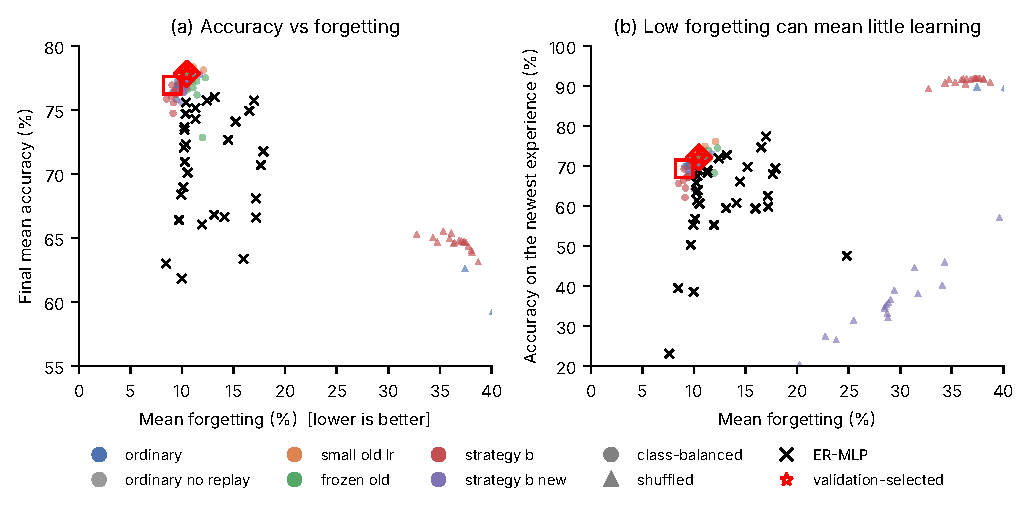
\includegraphics[width=\textwidth]{figures/fig_tradeoffs.pdf}
\caption{(a) Final accuracy versus forgetting and (b) newest-experience accuracy versus forgetting for \numPolyCandidatesThree\ polynomial candidates and \numErCandidates\ ER-MLP configurations (test seeds). \numBelowRange\ polynomial points below $55\%$ accuracy (mainly no-replay models) are outside panel (a). Red outlines: validation-selected polynomial settings. In panel (b), configurations with the lowest forgetting have the lowest newest-experience accuracy: they forget little because they learned little.}
\label{fig:tradeoffs}
\end{figure}

\subsection{Polynomial CIL versus experience replay (\RQ{1})}
Table~\ref{tab:h2h} places both methods on the same protocol, selection procedure and machine. The polynomial headline setting attains \numPolyBestAcc\% $\pm$ \numPolyBestAccSd\ accuracy with \numPolyBestForg\% forgetting; the validation-selected ER-MLP ($H{=}512$, $\eta{=}1$) attains \numErBestAcc\% $\pm$ \numErBestAccSd\ with \numErBestForg\% forgetting. That ER-MLP is more plastic (newest-experience accuracy \numErBestNew\% versus \numPolyBestNew\%) and forgets more. Against the ER-MLP chosen in hindsight on the test seeds ($H{=}512$, $\eta{=}0.3$, \numErHindAcc\%, \numErHindForg\% forgetting) the polynomial setting is still ahead, which makes the comparison conservative in the competitor's favour.

Table~\ref{tab:paired} gives paired differences, which are meaningful because both methods see the same experiences and exemplars for each seed. The polynomial setting is better in accuracy by \numPairedERMLPvalidationAccDiff\ points (95\% CI \numPairedERMLPvalidationAccLo\ to \numPairedERMLPvalidationAccHi) against the validation-selected ER-MLP and by \numPairedERMLPhindsightbAccDiff\ points (\numPairedERMLPhindsightbAccLo\ to \numPairedERMLPhindsightbAccHi) against the hindsight-best ER-MLP, in \numPairedERMLPhindsightbAccWins\ of \numPairs\ seeds, and it forgets less in every seed. The CIs are $t$-intervals over \numPairs\ seeds that vary only shuffling, replay selection and initialisation: they quantify optimiser noise, not dataset variability, and a sign test over seven seeds cannot go below $p=2/2^7\approx0.016$. We therefore read the result as a \emph{consistent small advantage on this protocol}, not as established superiority.

Cost does not separate the methods clearly. Per-run time is \numPolyBestTime\,s for the polynomial setting and \numErBestTime\,s for the ER-MLP with $H{=}512$, but the ER-MLP with $H{=}256$ reaches \numErFloorTradeAcc\% in \numErFloorTradeTime\,s with \numErFloorTradeParams\ parameters (polynomial: \numPolyBestParams). Counting the one-time feature construction of \numFeatureSeconds\,s, the polynomial method is clearly the more expensive of the two. The extra accuracy of \numPairedERMLPbesttradeAccDiff\ points over the $H{=}256$ model therefore comes with about $1.4\times$ the parameters and a fixed up-front cost.

\begin{table}[t]
\centering\scriptsize
\resizebox{\textwidth}{!}{\begin{tabular}{@{}llrrrrrr@{}}
\toprule
Setting & Configuration & Params & Memory & Acc.\ (\%) & Forg.\ (\%) & Newest (\%) & Time (s) \\
\midrule
\multicolumn{8}{@{}l}{\emph{Polynomial (expanding degrees $1,2,3,3,3$)}}\\
Highest accuracy (val.) & \texttt{frozen\_old}{,} $\eta=[2.5{,} 2.5{,} 10{,} 10]$ & 9{,}690 & 1{,}600 & 77.8{\scriptsize$\pm$0.4} & 10.5{\scriptsize$\pm$1.1} & 72.2 & 0.79 \\
Best trade-off (val.{,} literal) & \texttt{ordinary}{,} $\eta=[3{,} 3{,} 3{,} 3]$ & 9{,}690 & 1{,}600 & 76.9{\scriptsize$\pm$0.3} & 9.7{\scriptsize$\pm$0.8} & 70.6 & 0.91 \\
Lowest forgetting (val.{,} floor) & \texttt{strategy\_b}{,} $\eta=[12{,} 0.75{,} 0.75{,} 6]$ & 9{,}690 & 1{,}600 & 76.9{\scriptsize$\pm$0.3} & 9.0{\scriptsize$\pm$0.8} & 69.3 & 2.50 \\
Degree 1 throughout (val.-tuned $\eta$) & \texttt{ordinary}{,} $\eta=3$ & 170 & 1{,}600 & 66.8{\scriptsize$\pm$0.4} & 13.1{\scriptsize$\pm$0.8} & 59.0 & 0.16 \\
Degree 3 from the start (val.-tuned $\eta$) & \texttt{ordinary}{,} $\eta=10$ & 9{,}690 & 1{,}600 & 77.5{\scriptsize$\pm$0.6} & 12.5{\scriptsize$\pm$1.8} & 74.2 & 1.02 \\
No replay (core-selected $\eta$) & \texttt{ordinary\_no\_replay}{,} $\eta=[0.0025{,} 0.01{,} 0.02{,} 0.04]$ & 9{,}690 & 0 & 25.6{\scriptsize$\pm$0.0} & 82.4{\scriptsize$\pm$0.0} & 87.0 & 0.76 \\
\multicolumn{8}{@{}l}{\emph{ER-MLP (one hidden ReLU layer, plain SGD, replay)}}\\
Highest accuracy (val.) & $H=512${,} $\eta=1$ & 13{,}834 & 1{,}600 & 75.7{\scriptsize$\pm$1.1} & 17.0{\scriptsize$\pm$2.2} & 77.4 & 0.71 \\
Best trade-off (val.{,} literal) & $H=64${,} $\eta=0.1$ & 1{,}738 & 1{,}600 & 72.3{\scriptsize$\pm$0.3} & 10.4{\scriptsize$\pm$1.0} & 64.0 & 0.19 \\
Best trade-off (val.{,} floor) & $H=256${,} $\eta=0.3$ & 6{,}922 & 1{,}600 & 75.7{\scriptsize$\pm$0.5} & 12.4{\scriptsize$\pm$1.4} & 71.9 & 0.29 \\
Lowest forgetting (val.{,} floor) & $H=256${,} $\eta=0.1$ & 6{,}922 & 1{,}600 & 74.7{\scriptsize$\pm$0.3} & 10.3{\scriptsize$\pm$1.4} & 67.5 & 0.32 \\
Highest accuracy (hindsight{,} test) & $H=512${,} $\eta=0.3$ & 13{,}834 & 1{,}600 & 76.0{\scriptsize$\pm$0.9} & 13.2{\scriptsize$\pm$1.9} & 72.7 & 0.59 \\
Linear head (val.-tuned $\eta$) & linear head{,} $\eta=0.3$ & 170 & 1{,}600 & 66.8{\scriptsize$\pm$0.2} & 13.1{\scriptsize$\pm$0.5} & 59.5 & 0.12 \\
No replay & $H=512${,} $\eta=1$ & 13{,}834 & 0 & 18.8{\scriptsize$\pm$0.1} & 96.5{\scriptsize$\pm$0.2} & 93.9 & 0.67 \\
\bottomrule
\end{tabular}
}
\caption{Head-to-head on identical protocol, replay memory, seeds and machine (test seeds 3--9, 3 epochs). ``val.'' = ranked on validation; ``floor'' = within 2 points of the best accuracy; ``hindsight'' = ranked on the test seeds (optimistic). Params: parameters of the 10-way head. Memory: stored exemplars at the end.}
\label{tab:h2h}
\end{table}

\begin{table}[t]
\centering\scriptsize
\resizebox{\textwidth}{!}{\begin{tabular}{@{}lrrrr@{}}
\toprule
Polynomial (validation-selected) $-$ competitor & $\Delta$ acc.\ (pts) & 95\% CI & $\Delta$ forg.\ (pts) & 95\% CI \\
\midrule
ER-MLP, validation-selected ($H=512$, $\eta=1$) & +2.1 & [+1.1, +3.1] & -6.5 & [-8.3, -4.8] \\
ER-MLP, hindsight-best on test ($H=512$, $\eta=0.3$) & +1.8 & [+1.0, +2.6] & -2.7 & [-4.1, -1.4] \\
ER-MLP, best trade-off within accuracy floor ($H=256$, $\eta=0.3$) & +2.1 & [+1.5, +2.6] & -1.9 & [-2.9, -1.0] \\
\bottomrule
\end{tabular}
}
\caption{Paired differences (polynomial headline setting minus competitor) over the seven test seeds. Positive accuracy difference and negative forgetting difference favour the polynomial method. Seeds do not vary the data, so intervals understate dataset-level uncertainty.}
\label{tab:paired}
\end{table}

\begin{figure}[t]
\centering
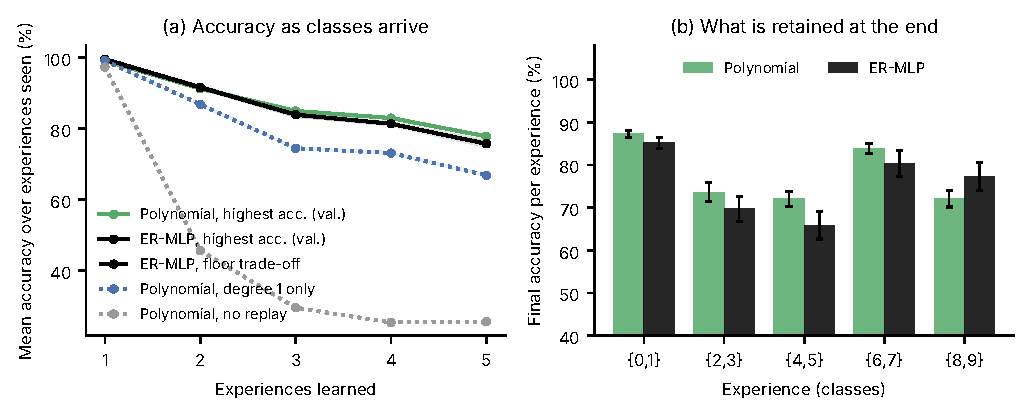
\includegraphics[width=\textwidth]{figures/fig_curves.pdf}
\caption{(a) Mean accuracy over experiences seen, after each experience (mean $\pm$ s.d.\ over seeds). (b) Final accuracy on each experience. The polynomial setting retains the middle experiences better; the ER-MLP is better on the newest one (\numPeErE\% versus \numPePolyE\%).}
\label{fig:curves}
\end{figure}

\subsection{Where does the effect come from? (\RQ{2})}
\paragraph{Capacity.} A degree-1 polynomial model is a linear softmax classifier and, as expected, matches the ER-MLP with a linear head (\numPolyLinearAcc\% versus \numErLinearAcc\%, forgetting \numPolyLinearForg\% versus \numErLinearForg\%), which also serves as a sanity check of the two implementations. Raising the degree to 3 from the start gives \numPolyFixedCapAcc\%, an increase of about 11 points. Polynomial capacity is the dominant factor.

\paragraph{Gradual expansion.} Expanding from degree 1 to 3 over the sequence does \emph{not} beat starting at degree 3. With a shared rate, the expanding schedule with plain replay gives \numCellOrdinaryCbSharedAcc\% accuracy and \numPolyTradeForg\% forgetting; degree 3 from the start, with its rate chosen on validation, gives \numPolyFixedCapAcc\% and \numPolyFixedCapForg\% forgetting. Expansion is thus associated with less forgetting (by about 2.8 points) and lower newest-experience accuracy (\numPolyTradeNew\% versus \numPolyFixedCapNew\%), that is, more stability and less plasticity, with no accuracy gain. This comparison is not perfectly balanced: the fixed-capacity model was tuned only over the shared-rate grid and without the update rules, which require ``old'' coefficients to exist.

\paragraph{Replay.} Without replay the polynomial model reaches only \numPolyNoReplayAcc\% (\numPolyNoReplayForg\% forgetting) and the ER-MLP \numErNoReplayAcc\%; both predict almost only the newest classes (newest-experience accuracy $\ge$ \numPolyNoReplayNew\%).

\paragraph{Sampling policy, update rule and per-degree rates.} Table~\ref{tab:cells} shows each update rule under both sampling policies. With class-balanced sampling the five replay-based rules lie within a narrow band (about 76--78\%), and the learning-rate vector chosen per degree changes accuracy by between \numPerDegreeGainCbMin\ and \numPerDegreeGainCbMax\ points relative to a shared rate. Under shuffled sampling accuracy collapses (median \numMedianShuffledAcc\% versus \numMedianClassBalancedAcc\%), with large seed-to-seed variance. In that regime the update rules do differ: \texttt{strategy\_b} (64.8\%) beats \texttt{ordinary} (\numCellOrdinaryShSharedAcc\%) and \texttt{frozen\_old} (\numCellFrozenOldShSharedAcc\%) with a shared rate. A reading consistent with these numbers, though not proved by them, is that much of what the update rules and large per-degree rates achieve under shuffled sampling is compensation for class imbalance (about 5\,900 current examples versus 200 stored per old class in the last experience), which class-balanced sampling removes directly. The headline setting is not better than the shared-rate cells (\numCellFrozenOldCbSharedAcc\% for \texttt{frozen\_old}, 78.0\% for \texttt{small\_old\_lr}); the differences among these cells are within seed noise, so the per-degree vector is not what separates the polynomial method from the ER-MLP, and the ranking of the top polynomial cells is not resolved by this study.

\begin{table}[t]
\centering\scriptsize
\resizebox{\textwidth}{!}{\begin{tabular}{@{}llrrrrlrrrr@{}}
\toprule
 & & \multicolumn{3}{c}{Shared rate $\eta$} & & \multicolumn{4}{c}{Per-degree vector (validation-selected)} & \\
\cmidrule(lr){3-5}\cmidrule(lr){7-10}
Update rule & Sampling & $\eta$ & Acc.\ (\%) & Forg.\ (\%) & & $\eta$ (deg.\ 0--3) & Acc.\ (\%) & Forg.\ (\%) & $t$ (s) \\
\midrule
\texttt{ordinary} & \texttt{class\_balanced} & 3 & 76.9{\scriptsize$\pm$0.3} & 9.7{\scriptsize$\pm$0.8} & & [0.75, 1.5, 1.5, 6] & 77.3{\scriptsize$\pm$0.3} & 9.6{\scriptsize$\pm$0.8} & 0.79 \\
\texttt{ordinary} & \texttt{shuffled} & 30 & 56.8{\scriptsize$\pm$7.2} & 43.7{\scriptsize$\pm$8.8} & & [30, 30, 30, 120] & 62.6{\scriptsize$\pm$8.1} & 37.4{\scriptsize$\pm$11.0} & 0.87 \\
\addlinespace[2pt]
\texttt{ordinary\_no\_replay} & \texttt{class\_balanced} & 0.01 & 22.1{\scriptsize$\pm$0.0} & 86.5{\scriptsize$\pm$0.0} & & [0.0025, 0.01, 0.02, 0.04] & 25.6{\scriptsize$\pm$0.0} & 82.4{\scriptsize$\pm$0.0} & 0.76 \\
\texttt{ordinary\_no\_replay} & \texttt{shuffled} & 0.01 & 22.1{\scriptsize$\pm$0.0} & 86.9{\scriptsize$\pm$0.0} & & [0.0025, 0.0025, 0.01, 0.04] & 26.4{\scriptsize$\pm$0.0} & 81.5{\scriptsize$\pm$0.0} & 0.72 \\
\addlinespace[2pt]
\texttt{small\_old\_lr} & \texttt{class\_balanced} & 10 & 78.0{\scriptsize$\pm$0.4} & 10.5{\scriptsize$\pm$1.3} & & [20, 10, 10, 10] & 77.8{\scriptsize$\pm$0.5} & 10.1{\scriptsize$\pm$2.0} & 0.87 \\
\texttt{small\_old\_lr} & \texttt{shuffled} & 10 & 54.8{\scriptsize$\pm$5.0} & 48.7{\scriptsize$\pm$6.1} & & [2.5, 40, 20, 40] & 58.5{\scriptsize$\pm$6.5} & 42.9{\scriptsize$\pm$7.3} & 0.74 \\
\addlinespace[2pt]
\texttt{frozen\_old} & \texttt{class\_balanced} & 10 & 77.6{\scriptsize$\pm$0.5} & 10.8{\scriptsize$\pm$1.5} & & [2.5, 2.5, 10, 10] & 77.8{\scriptsize$\pm$0.4} & 10.5{\scriptsize$\pm$1.1} & 0.79 \\
\texttt{frozen\_old} & \texttt{shuffled} & 30 & 46.2{\scriptsize$\pm$7.1} & 55.7{\scriptsize$\pm$8.0} & & [15, 30, 30, 30] & 47.6{\scriptsize$\pm$6.3} & 55.1{\scriptsize$\pm$6.3} & 0.76 \\
\addlinespace[2pt]
\texttt{strategy\_b} & \texttt{class\_balanced} & 3 & 76.4{\scriptsize$\pm$0.2} & 9.4{\scriptsize$\pm$0.7} & & [12, 0.75, 0.75, 6] & 76.9{\scriptsize$\pm$0.3} & 9.0{\scriptsize$\pm$0.8} & 2.50 \\
\texttt{strategy\_b} & \texttt{shuffled} & 30 & 64.8{\scriptsize$\pm$0.8} & 37.1{\scriptsize$\pm$1.3} & & [120, 120, 120, 60] & 65.3{\scriptsize$\pm$1.0} & 32.7{\scriptsize$\pm$2.1} & 2.47 \\
\addlinespace[2pt]
\texttt{strategy\_b\_new} & \texttt{class\_balanced} & 10 & 77.1{\scriptsize$\pm$0.2} & 10.3{\scriptsize$\pm$0.7} & & [5, 5, 2.5, 10] & 76.7{\scriptsize$\pm$0.3} & 9.8{\scriptsize$\pm$0.7} & 2.65 \\
\texttt{strategy\_b\_new} & \texttt{shuffled} & 0.03 & 53.5{\scriptsize$\pm$2.0} & 28.7{\scriptsize$\pm$2.3} & & [0.12, 0.12, 0.03, 0.0075] & 50.5{\scriptsize$\pm$3.3} & 16.7{\scriptsize$\pm$1.7} & 2.54 \\
\addlinespace[2pt]
\bottomrule
\end{tabular}
}
\caption{Update rule $\times$ sampling policy: shared-rate reference versus the validation-selected per-degree vector (test seeds 3--9, 3 epochs; $t$ re-measured here for the selected vector).}
\label{tab:cells}
\end{table}

\subsection{Training budget (\RQ{4})}
With ten epochs (Table~\ref{tab:epochs}, no re-selection) the polynomial setting improves to \numPolyTenAcc\% (forgetting \numPolyTenForg\%), whereas the ER-MLPs do not improve in accuracy and forget more (for example, forgetting rises from \numErFloorTradeForg\% to about 17\% for $H{=}256$). The best ER-MLP at ten epochs reaches \numErTenBestAcc\%, so the gap of roughly 2.6 points persists. Time grows about twofold for the polynomial setting and about three- to fourfold for the ER-MLPs (Table~\ref{tab:epochs}). Because rates were selected for three epochs, a re-tuned ER-MLP might do better at ten; we did not test this.

\begin{table}[t]
\centering\scriptsize
\resizebox{\textwidth}{!}{\begin{tabular}{@{}llrrrrrr@{}}
\toprule
Method & Configuration & Acc.\ 3 ep. & Acc.\ 10 ep. & Forg.\ 3 ep. & Forg.\ 10 ep. & Time 3 ep. & Time 10 ep. \\
\midrule
Polynomial & \texttt{frozen\_old}, $\eta=[2.5, 2.5, 10, 10]$ & 77.8{\scriptsize$\pm$0.4} & 78.6{\scriptsize$\pm$0.5} & 10.5{\scriptsize$\pm$1.1} & 11.9{\scriptsize$\pm$1.1} & 0.79 & 1.57 \\
ER-MLP & $H=512$, $\eta=1$ & 75.7{\scriptsize$\pm$1.1} & 74.2{\scriptsize$\pm$1.3} & 17.0{\scriptsize$\pm$2.2} & 23.0{\scriptsize$\pm$2.0} & 0.71 & 2.01 \\
ER-MLP & $H=512$, $\eta=0.3$ & 76.0{\scriptsize$\pm$0.9} & 76.0{\scriptsize$\pm$0.7} & 13.2{\scriptsize$\pm$1.9} & 17.6{\scriptsize$\pm$1.2} & 0.59 & 1.94 \\
ER-MLP & $H=256$, $\eta=0.3$ & 75.7{\scriptsize$\pm$0.5} & 75.6{\scriptsize$\pm$0.6} & 12.4{\scriptsize$\pm$1.4} & 16.8{\scriptsize$\pm$1.2} & 0.29 & 1.05 \\
\bottomrule
\end{tabular}
}
\caption{Three versus ten epochs per experience, without re-selection (test seeds 3--9).}
\label{tab:epochs}
\end{table}

\subsection{Does validation selection transfer? (\RQ{5})}
Across the \numCandidatesValidation\ validation candidates, validation and test accuracy are almost perfectly rank-correlated (Spearman $\rho=\numSpearmanAcc$; forgetting $\rho=\numSpearmanForg$), but this is driven by the wide range that includes no-replay and unstable candidates; among the 60 best candidates it falls to $\rho=\numSpearmanAccTop$. Test accuracy is on average \numMeanAccGap\ points higher than validation accuracy, plausibly because the validation models are fitted to 90\% of the training data and the two splits are not equally difficult; we did not investigate this. The validation-selected setting is \numRegret\ points below the best three-epoch candidate in hindsight, and the hindsight best overall (ten epochs, \numPolyTenAcc\%) differs from the validation-selected one only through the extra epochs. The optimism of selecting on test is thus small here, but it is not zero, and it is why we base all claims on the validation ranking.

\begin{figure}[t]
\centering
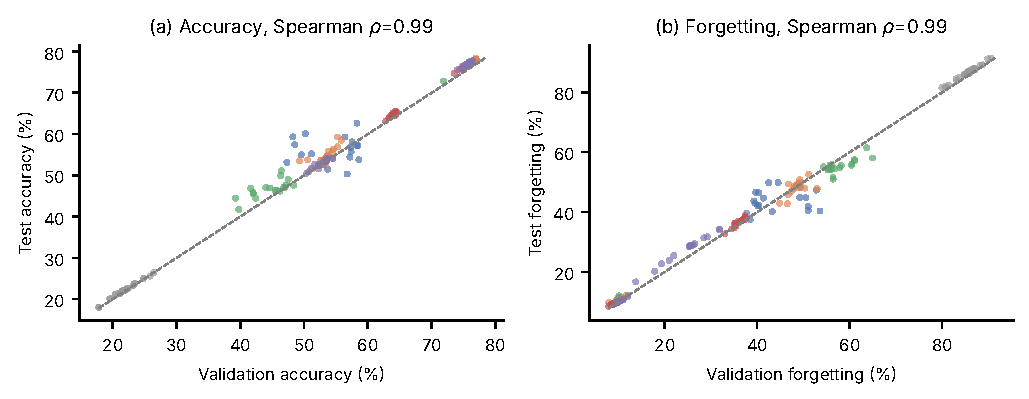
\includegraphics[width=\textwidth]{figures/fig_transfer.pdf}
\caption{Validation versus test (a) accuracy and (b) forgetting for all three-epoch polynomial candidates, coloured by update rule. The dashed line is $y=x$.}
\label{fig:transfer}
\end{figure}

\section{Discussion}
\paragraph{Is polynomial CIL ``an answer''?}
On this protocol it is a competitive and modestly better answer than a replay MLP of comparable size, with lower forgetting and a consistent paired advantage across seeds. It is not demonstrated to be an answer \emph{for the reason it was proposed}. The method's three distinguishing ingredients (incremental expansion, protective update rules, per-degree learning rates) contribute little or nothing measurable once class-balanced replay is used; the strong effects are polynomial capacity, replay and balanced sampling. A fair summary is that a degree-3 polynomial head on a 16-dimensional projection is a well-conditioned, cheap-to-train classifier that suits replay-based CIL, and that gradual expansion trades some plasticity for stability.

\paragraph{Why might the polynomial head forget less?}
The ER-MLP adapts a shared hidden representation to every experience, whereas a polynomial head with a fixed feature map changes only a linear readout of fixed features; this is a plausible reason for lower forgetting and lower plasticity (Fig.~\ref{fig:curves}b), but the present study does not isolate it (for example by freezing the MLP's hidden layer or by adding random-feature baselines of matching width).

\paragraph{What ``best'' means.}
The criteria produce four different winners, two of which are degenerate (Fig.~\ref{fig:tradeoffs}b). A benchmark should therefore report a Pareto set with newest-experience accuracy, as the accompanying results do, and not a single scalar; the trade-off score is useful for presenting one default, provided its weighting is stated.

\paragraph{Open questions.}
Does the advantage persist with higher-dimensional inputs, where the number of monomials explodes and the 16-dimensional projection is not available? Is it a property of the head or of the fixed projection? How do stronger CIL methods (iCaRL-style exemplar classifiers, gradient-projection methods) compare? Would a tuned learning-rate schedule or weight decay remove the ER-MLP's disadvantage? Would a different task order or a different number of classes per experience change the ranking of update rules?

\subsection*{Threats to validity and limitations}
\begin{itemize}
\item \textbf{One dataset and a weak input representation.} Split MNIST on a 16-dimensional random projection yields about 78\% accuracy; absolute numbers are not comparable to results using full-resolution inputs and deeper networks. Additional datasets will be needed if reviewers ask for them.
\item \textbf{One competitor family.} Only an ER-MLP was run. EWC, LwF and other methods were not, so the comparison does not establish a position among CIL methods.
\item \textbf{Unequal search effort.} The polynomial method was tuned over \numPolyCandidatesThree\ candidates (including structural choices), the ER-MLP over \numErCandidates\ (width and rate). The ER-MLP's validation-selected configuration sits at the upper edge of the width grid ($H{=}512$; its rate is interior), so a wider search could raise it.
\item \textbf{Seed variance only.} Seeds do not vary the data split or projection.
\item \textbf{Timing.} Single machine, one core, sub-second to few-second runs; excluding polynomial feature construction favours the polynomial method.
\item \textbf{Numerical reproducibility.} Re-running \numReproChecks\ polynomial settings against the stored core results reproduced \numReproExact\ of them bit-for-bit. All class-balanced settings agree to $\le 1.2\times10^{-4}$; the largest differences ($\le \numReproMaxDiff$) occur for shuffled sampling with rates $\ge30$, where training is unstable and floating-point differences between machines are amplified. Conclusions rest on the class-balanced settings.
\item \textbf{Fixed-capacity ablation.} It was tuned with a shared rate only.
\end{itemize}

\section{Conclusion}
Under one controlled protocol, polynomial CIL with class-balanced replay is a small but consistent improvement over a tuned experience-replay MLP in accuracy and forgetting, at comparable per-run cost once features are available. The improvement is attributable chiefly to polynomial capacity and balanced replay, not to incremental expansion, update rules or per-degree learning rates, which the ablations leave unsupported as sources of accuracy. The study's main methodological lesson is that single-number ``best'' claims (lowest forgetting, smallest time, best trade-off) are fragile or degenerate and should be replaced by validation-based Pareto reporting.

\appendix
\section{Reproducibility}
\begin{itemize}
\item \textbf{Core package} \texttt{polynomial\_cl}: commit \texttt{b0b917ee240db7a7ea7d78cb4bf21754e99d554b} of the checkout supplied for this study, with uncommitted working-tree changes (21 modified files). The benchmark's imports were updated to the refactored core API (\texttt{polynomial\_cl.continual}, \texttt{polynomial\_cl.data}); the core was not modified. After this change the adapter reproduces the stored seed-3 result of the combined per-degree setting exactly (accuracy 0.7734281931972611, forgetting 0.09086581818480258).
\item \textbf{Stored study results}: produced by \texttt{experiments/run\_per\_degree\_study.sh} of the core (selection seeds 0--2, test seeds 3--9).
\item \textbf{Analysis} (wall time is not stored in the result JSON; it is read from the logs and each log line is cross-checked against the JSON run before use):
\begin{verbatim}
python tools/analyze_per_degree_study.py \
  --results-dir <core>/results/per_degree \
  --out-json results/analysis/per_degree_analysis.json \
  --out-md   results/analysis/per_degree_analysis.md \
  --out-csv  results/analysis/per_degree_candidates.csv
\end{verbatim}
\item \textbf{Comparison} (resumable; every run, failed ones included, is appended to \texttt{runs.jsonl}):
\begin{verbatim}
python tools/run_comparison_study.py \
  --analysis results/analysis/per_degree_analysis.json \
  --core-results <core>/results/per_degree \
  --out-dir results/comparison
\end{verbatim}
\item \textbf{Paper assets} (all tables, figures and quoted numbers are generated here):
\begin{verbatim}
python tools/build_paper_assets.py \
  --analysis results/analysis/per_degree_analysis.json \
  --comparison results/comparison --out paper
\end{verbatim}
\end{itemize}

\begin{thebibliography}{99}\small
\bibitem{mccloskey1989} M.~McCloskey and N.~J.~Cohen. Catastrophic interference in connectionist networks. \emph{Psychology of Learning and Motivation}, 24:109--165, 1989.
\bibitem{vandeven2019} G.~M.~van de Ven and A.~S.~Tolias. Three scenarios for continual learning. arXiv:1904.07734, 2019.
\bibitem{hsu2018} Y.-C.~Hsu, Y.-C.~Liu, A.~Ramasamy and Z.~Kira. Re-evaluating continual learning scenarios: a categorization and case for strong baselines. arXiv:1810.12488, 2018.
\bibitem{chaudhry2019tiny} A.~Chaudhry et al. On tiny episodic memories in continual learning. arXiv:1902.10486, 2019.
\bibitem{rebuffi2017} S.-A.~Rebuffi, A.~Kolesnikov, G.~Sperl and C.~H.~Lampert. iCaRL: incremental classifier and representation learning. In \emph{CVPR}, 2017.
\bibitem{prabhu2020} A.~Prabhu, P.~H.~S.~Torr and P.~K.~Dokania. GDumb: a simple approach that questions our progress in continual learning. In \emph{ECCV}, 2020.
\bibitem{chaudhry2018riemannian} A.~Chaudhry, P.~K.~Dokania, T.~Ajanthan and P.~H.~S.~Torr. Riemannian walk for incremental learning: understanding forgetting and intransigence. In \emph{ECCV}, 2018.
\bibitem{delange2021} M.~De~Lange et al. A continual learning survey: defying forgetting in classification tasks. \emph{IEEE TPAMI}, 44(7):3366--3385, 2022.
\bibitem{diaz2018} N.~D\'iaz-Rodr\'iguez, V.~Lomonaco, D.~Filliat and D.~Maltoni. Don't forget, there is more than forgetting: new metrics for continual learning. arXiv:1810.13166, 2018.
\bibitem{farquhar2018} S.~Farquhar and Y.~Gal. Towards robust evaluations of continual learning. arXiv:1805.09733, 2018.
\bibitem{kirkpatrick2017} J.~Kirkpatrick et al. Overcoming catastrophic forgetting in neural networks. \emph{PNAS}, 114(13):3521--3526, 2017.
\bibitem{zenke2017} F.~Zenke, B.~Poole and S.~Ganguli. Continual learning through synaptic intelligence. In \emph{ICML}, 2017.
\bibitem{li2018} Z.~Li and D.~Hoiem. Learning without forgetting. \emph{IEEE TPAMI}, 40(12):2935--2947, 2018.
\bibitem{lopezpaz2017} D.~Lopez-Paz and M.~Ranzato. Gradient episodic memory for continual learning. In \emph{NeurIPS}, 2017.
\bibitem{farajtabar2020} M.~Farajtabar, N.~Azizan, A.~Mott and A.~Li. Orthogonal gradient descent for continual learning. In \emph{AISTATS}, 2020.
\bibitem{saha2021} G.~Saha, I.~Garg and K.~Roy. Gradient projection memory for continual learning. In \emph{ICLR}, 2021.
\bibitem{mai2022} Z.~Mai et al. Online continual learning in image classification: an empirical survey. \emph{Neurocomputing}, 469:28--51, 2022.
\bibitem{ivakhnenko1971} A.~G.~Ivakhnenko. Polynomial theory of complex systems. \emph{IEEE Trans.\ Systems, Man, and Cybernetics}, 1(4):364--378, 1971.
\bibitem{chang2010} Y.-W.~Chang, C.-J.~Hsieh, K.-W.~Chang, M.~Ringgaard and C.-J.~Lin. Training and testing low-degree polynomial data mappings via linear SVM. \emph{JMLR}, 11:1471--1490, 2010.
\bibitem{chrysos2022} G.~G.~Chrysos et al. Deep polynomial neural networks. \emph{IEEE TPAMI}, 44(8):4021--4034, 2022.
\end{thebibliography}
\end{document}
